    \documentclass[10pt]{article}
    \usepackage{fancyhdr, amsmath, amsthm, amssymb, mathtools, lastpage, hyperref, enumerate, graphicx, setspace, wasysym, listings}
    \usepackage[margin=1in]{geometry}
    \newcommand{\scinot}[2]{#1\times10^{#2}}
    \newcommand{\bra}[1]{\left<#1\right|}
    \newcommand{\ket}[1]{\left|#1\right>}
    \newcommand{\dotp}[2]{\left<#1\,\middle|\,#2\right>}
    \newcommand{\rd}[2]{\frac{\mathrm{d}#1}{\mathrm{d}#2}}
    \newcommand{\pd}[2]{\frac{\partial#1}{\partial#2}}
    \newcommand{\rtd}[2]{\frac{\mathrm{d}^2#1}{\mathrm{d}#2^2}}
    \newcommand{\ptd}[2]{\frac{\partial^2 #1}{\partial#2^2}}
    \newcommand{\norm}[1]{\left|\left|#1\right|\right|}
    \newcommand{\abs}[1]{\left|#1\right|}
    \newcommand{\pvec}[1]{\vec{#1}^{\,\prime}}
    \newcommand{\tensor}[1]{\overleftrightarrow{#1}}
    \let\Re\undefined
    \let\Im\undefined
    \newcommand{\ang}[0]{\text{\AA}}
    \newcommand{\mum}[0]{\upmu \mathrm{m}}
    \DeclareMathOperator{\Re}{Re}
    \DeclareMathOperator{\Im}{Im}
    \DeclareMathOperator{\Log}{Log}
    \DeclareMathOperator{\Arg}{Arg}
    \DeclareMathOperator{\Tr}{Tr}
    \DeclareMathOperator{\E}{E}
    \DeclareMathOperator{\Var}{Var}
    \DeclareMathOperator*{\argmin}{argmin}
    \DeclareMathOperator*{\argmax}{argmax}
    \DeclareMathOperator{\sgn}{sgn}
    \newcommand{\expvalue}[1]{\left<#1\right>}
    \usepackage[font=scriptsize]{subcaption}
    \everymath{\displaystyle}

\begin{document}

\pagestyle{fancy}
\rhead{Nancy Cao, Joanne Li, Yubo Su --- CS155 Sentiment Analysis}
\cfoot{\thepage/\pageref{LastPage}}

\title{Machine Learning \& Data Mining\\
      Caltech CS/CNS/EE 155 \\[1pt]
      Sentiment Analysis}
\author{Nancy Cao, Joanne Li, Yubo Su}
\date{February 11, 2016}
\maketitle

\begin{abstract}
In this study, we attempt to predict the sentiment of a speech based on a bag of words representation over 1000 common, stemmed words. A highly sparse training set of $4189$ speeches was used in order to predict sentiments on a testing dataset of $1000$ speeches. The final iteration of the model was able to attain $66.6, 66.7\%$ accuracy on both public and private components of the testing dataset respectively, indicating that no overfitting to the public dataset is observed. The final two submitted models comprised a bag of random models with slightly randomized parameters and a bag that aggregated models only that increased a 5-fold cross validation score.
\end{abstract}

\section{Overview}

The objective of the project was to determine a machine learning model that would be able to predict speech sentiment based on a bag-of-words representation. The codebase was written entirely using Python 3.5.1 using learning routines from Python-scikit-learn 0.17-2, though with wrappers implemented by the group members. Our code is publically available online \footnote{\url{https://github.com/yubo56/CS155SentimentAnalysis}}. The work distribution within the group was:
\begin{itemize}
    \item Nancy Cao -- Responsible for management of group and assisted with planning remotely.
    \item Joanne Li -- Responsible for model selection and training models to obtain results.
    \item Yubo Su -- Responsible for model iteration and performance characterization.
\end{itemize}

The primary challenge incurred was a strange accident where only within 12 hours of the deadline did we obtain the correct data. The initial data were downloaded on Jan. 22 and were in the same format as the correct training/testing dataset but contained different values. Thus, even enormous \texttt{RandomForestClassifier}s yielded performance statistically consistent with guessing. Only four submissions were made with the correct data, one of which was a test submission.

The robustness of our approach is supported by our ability to converge to a leading score on the public scoreboard with only three attempts.

\section{Data Manipulation}

We implemented a term frequency-inverse document frequency (tf-idf) transformation, using the built in routine \texttt{sklearn.feature\_extraction.text.TfidfTransformer()} to perform the transformation. The class of tf-idf transformations is considered to be a heuristic that improves performance of learning algorithms on textual collections, as it weights words unique to a document more strongly than words shared across all documents. We also observed a small performance increase in implementing the tf-idf transformation at various stages of the testing process.

\section{Learning Algorithm}

Numerous initial learning algorithms were employed in an attempt to better characterise the fitting process and discover what was wrong with our fitting procedure, before we discovered the correct dataset. They are not reported here in the interest of brevity, though a more complete prediction history can be found on the project GitHub webpage. We present below only the learning algorithms that were in consideration for the final predictions.

\begin{enumerate}[a)]
    \item sklearn default \texttt{RandomForestClassifier}

        Other than custom ensemble methods, running the default sklearn random forest classifier was our primary mode of out-of-the-box machine learning. We quickly did a parameter scan using 5-fold cross validation to perform hyperparameter optimization on the maximum number of features per tree and the minimum number of samples required to split a tree node.

        The ultimate best performance of a random forest classifier was $0.660, 0.670$ on the public/private datasets respectively, using $70000$ trees.
    \item Random ensemble.

        We created a custom class that could automatically take a given model and train the model, predict on a test set and append the predictions to a cumulative prediction. The ensemble's prediction on the test data was then just the majority prediction of the ensemble. The ensemble was allowed to run until the majority prediction converged, thus averaging over any stochastic over/underfitting introduced by individual models.

        A wide selection of models of various expected predictive capacity was chosen to maximize robustness of the ensemble with respect to dataset. By including both over and underfitting models in the ensemble, the average behavior of the model is insulated against large changes in how well the sampled data represent the full range of inputs. 
        
        Each model below was individually subjected to the same 5-fold cross validation scan as above for random forests for hyperparameter optimization. A random noise was then introduced around the best parameter before adding to the ensemble to introduce noise to our classification and further increase the robustness of our sample to non-representative sampling. The models used and their chosen hyperparameter ranges are:
        \begin{enumerate}[i.]
            \item Adaboost --- 100 estimators, learning rate $0.03 \pm 0.02$.

            \item Bagging Classifier --- 100 estimators, maximum number of features $0.5 \pm 0.2$ of total number of features, maximum number of samples $0.7 \pm 0.2$ number of samples.

            \item Decision Tree Classifier --- 5 minimum samples to split, maximum number of features $0.64 \pm 0.02$.

            \item Gradient Boosting Classifier --- 100 estimators, 7 minimum samples to split, 6 maximum depth of tree, subsampling $0.7 \pm 0.3$
            \item Random Forest Classifier --- 450 estimators, $0.0420^{0.16}_{0.04}$ of total features, 7 samples to split.
            \item Random Forest Classifier --- 100 estimators, $0.0420^{0.32}_{0.2}$ of total features, 7 samples to split.

            \item SGD Classifier --- Hinge loss, $\alpha$ regularizer $0.005631 \pm 0.005$
            \item Linear SVM --- $C$ regularizer $0.06 \pm 0.5$

            \item Linear SVM --- $C$ regularizer $550 \pm 450$.
    \end{enumerate}

        Note that some parameters were chosen with different upper and lower bounds to allow for increased variance when the parameter is too close to its extremal allowed value.

        The ultimate best performance of this random ensemble was $0.666, 0.667$ on the public, private datasets respectively.

    \item CV-optimizing random ensemble

        A modification to the above ensemble was added such that cross-validation scores were stored dynamically and an additional model bagged only if it improved the aggregate 5-fold CV score. Otherwise, the hyperparameter space of allowed models was chosen to be the same as above. Unfortunately, there was insufficient time to allow this model to run until convergence, but the ensemble exhibited strong barriers to entry even after just 15 models in the bag, showing that we'd already managed to outperform the large majority of our parameter space with just a few models.

        The best performance of this ensemble was $0.666, 0.667$ on the public and private datasets respectively.

\end{enumerate}

Please note that many earlier iterations of models made their way into the final ensemble models as hyperparameter-tuned contributions to the bagged prediction. For instance, our SGD, SVM classifiers were both initial models that were submitted, but they were still used in the ensemble methods above.

\section{Model Selection}

The final two models were chosen to be the two ensemble bagging methods, both because they seemed to maximize performance of the three strongly predictive models that were run on the correct dataset and because they should have maximally decorreleated from any sampling bias or representation bias in the training dataset by allowing for over/underfitting and predictions from various different models each exhibiting various systematic training tendencies. 

We can see the robustness of our models by noting that the private and public performance scores are significantly closer $\sim 0.001$ than on the random forest $\sim 0.01$.

\section{Conclusion}

\subsection{Performance}

Our model was able to insulate extremely strongly against different testing datasets (performing to within $0.1\%$ on the public/private components of the testing dataset). We were also able to observe quite strong predictive capacity, and therefore we believe the performance of our model is satisfactory and within expectation.

While our model dropped significantly in relative accuracy when examining the public and private dataset, the discrepancy can clearly be attributed to a correlated sampling between the private dataset and the training set. While our accuracy remained very robust to different testing datasets, all other groups' accuracies improved significantly on the private testing dataset. While this can be attributed to noise, the strongly correlated effect suggests an underlying co-variance in the sampling of the two datasets. Our model, by maximally decorrelating estimates between bag contributions via randomized hyperparemeters and randomized parameter models, is able to insulate against this systematic bias. Should the co-variance have been in the other direction, such that overfitted predictions to the training data perform \emph{worse} on the private training data, we would have expected to perform better in comparison to other groups under the private than public training data.

Even as this argument is unjustified without extra data points, what is clear is that our performance penalty relative to the rest of the class cannot have been a result of overfitting to the public training data as we only made four submissions with the correct testing set.

\subsection{Possible Improvements}

A complete run of the CV-optimizing random ensemble would have probably improved our score, as with only 15 classifiers in the ensemble we would still expect to see large variance in the performance of the classifier, while with a more optimized ensemble it would both have better learned features in the dataset and be more robust to perturbations.

Another possible improvement is a weighted contribution to the prediction score within the ensemble methods. For instance, when classifiers that are already ensemble-like in nature e.g. random forests are added to the ensemble, their predictions should be weighted more strongly than single decision trees, as they represent the prediction of multiple decision trees. The exact weighting would need to be further investigated, possibly another tunable hyperparameter.

\appendix

\section{Plots of CV hyperparameter optimization}

Before discovering skikit's own grid hyperparameter space explorer, a custom parameter space exploration was coded based on 5-fold CV score distributions. Some examples of these results are plotted below in \autoref{fig:aaa}. The result to draw from this particular hyperoptimization would have been that the fractional number of features to draw into the random forest is $\approx 0.38$ because it maximizes the mean CV score while not incurring too much extra variance. Note the graphs are a bit noisy, rendering this sort of technique somewhat unreliable.
\begin{figure}[!h]
    \centering
    \begin{subfigure}{0.3\textwidth}
        \centering
        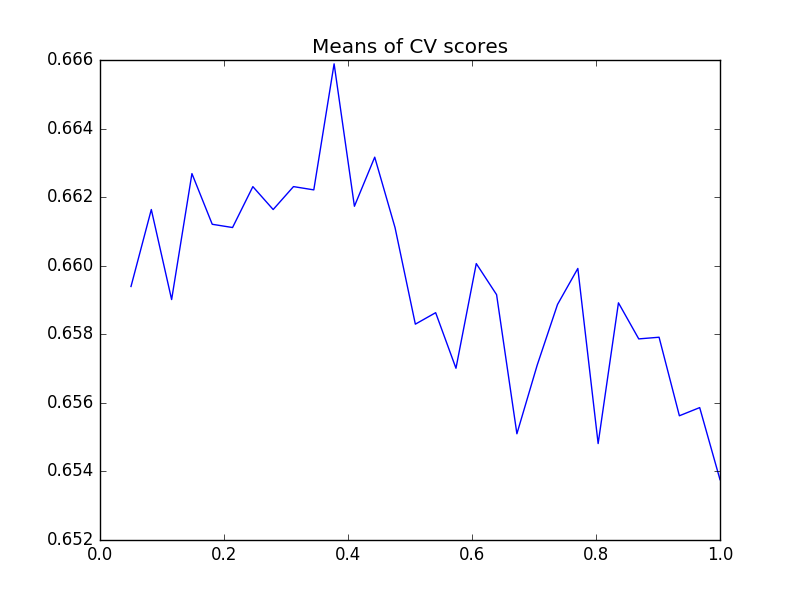
\includegraphics[width=\textwidth]{images/testRFMaxFeatMeans.png}
        \caption{Plot of mean CV score as function of fractional maximum number of features.}
    \end{subfigure}
    \begin{subfigure}{0.3\textwidth}
        \centering
        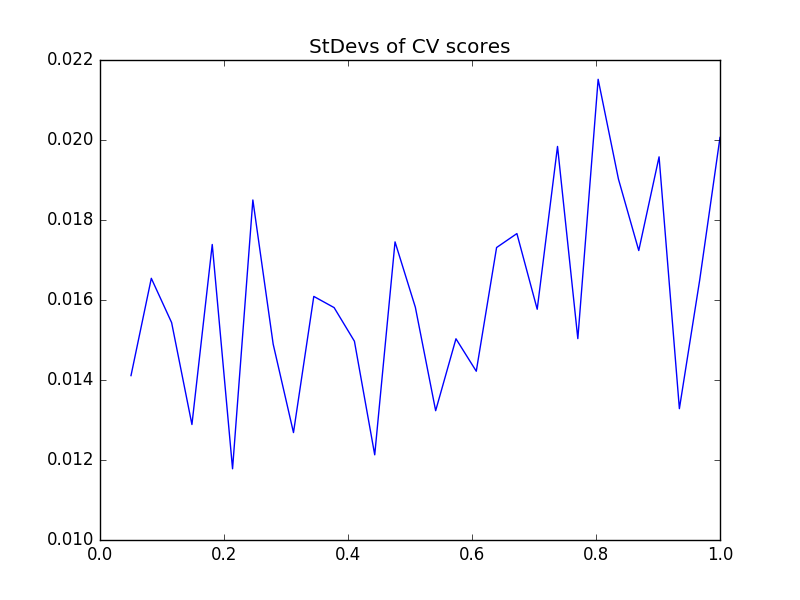
\includegraphics[width=\textwidth]{images/testRFMaxFeatStDevs.png}
        \caption{Plot of standard deviation of CV score as function of fractional maximum number of features.}
    \end{subfigure}
    \caption{Example of hyperparameter optimization using CV scores for random forest, $100$ sub-trees. Before going to sklearn's \texttt{GridSearchCV}.}
    \label{fig:aaa}
\end{figure}

\end{document}

